% Blocks 3a + 3b — recurrence per-channel + unrolled across time.
% Full-width standalone. Compile:  pdflatex arch_expand_recurrence.tex

\documentclass[tikz,border=8pt]{standalone}
\usepackage{tikz}
\usepackage{amsmath,amssymb}
\usepackage{xcolor}
\usetikzlibrary{positioning,arrows.meta,calc,fit,backgrounds}

\newcommand{\bm}{\mathbf{m}}
\newcommand{\bs}{\mathbf{s}}
\newcommand{\bh}{\mathbf{h}}

\definecolor{cBipolar}{HTML}{2C5282}
\definecolor{cBipolarLite}{HTML}{EBF4FF}
\definecolor{cCont}{HTML}{B7791F}
\definecolor{cContLite}{HTML}{FFF8E6}
\definecolor{cOp}{HTML}{2D3748}
\definecolor{cPanelBg}{HTML}{FAFBFC}
\definecolor{cPanelBorder}{HTML}{CBD5E0}
\definecolor{cArrow}{HTML}{1A202C}

\tikzset{
  block/.style={draw=cPanelBorder, fill=cPanelBg, thick, rounded corners=6pt,
                inner sep=8pt, minimum width=170mm},
  blockTitle/.style={font=\bfseries\normalsize, anchor=north west, inner sep=6pt},
  cellPos/.style={draw=cBipolar!50, fill=cBipolarLite, font=\small,
                  minimum width=9mm, minimum height=8mm, inner sep=0pt},
  cellNeg/.style={draw=cBipolar!50, fill=cBipolar!18, font=\small,
                  minimum width=9mm, minimum height=8mm, inner sep=0pt},
  cellCont/.style={draw=cCont!60, fill=cContLite, font=\small,
                   minimum width=13mm, minimum height=8mm, inner sep=0pt},
  op/.style={draw=cOp, fill=white, thick, circle, inner sep=1.4pt,
             font=\small, minimum size=7mm},
  flow/.style={-{Stealth[length=2.2mm]}, thick, draw=cArrow},
  flowSm/.style={-{Stealth[length=1.8mm]}, semithick, draw=cArrow!85},
  lbl/.style={font=\scriptsize\itshape, text=black!65, align=center},
  matlbl/.style={font=\scriptsize, text=cBipolar!85!black, align=center},
}

\begin{document}
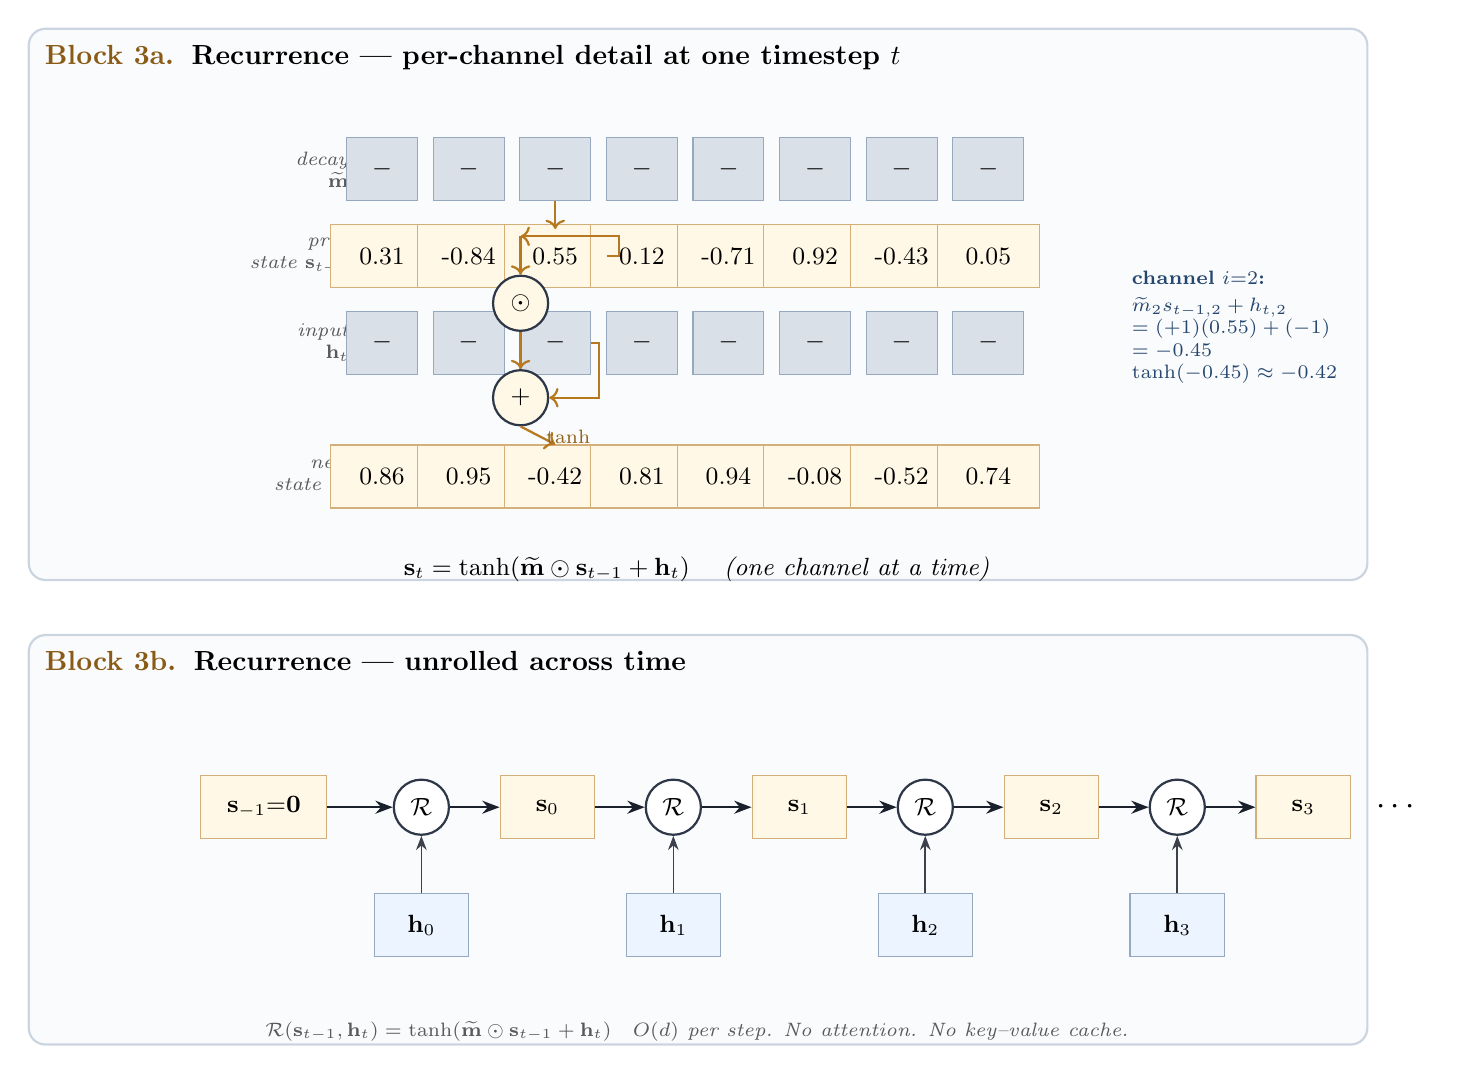
\begin{tikzpicture}

% ========== BLOCK 3a: PER-CHANNEL ==========
\node[block, minimum height=70mm, anchor=north west] (B3a) at (0,0) {};
\node[blockTitle] at (B3a.north west)
  {\textcolor{cCont!75!black}{Block 3a.}\;\;Recurrence --- per-channel detail at one timestep $t$};

\begin{scope}[shift={(4.5,-1.8)}]
  \node[lbl, anchor=east, align=right] at (-0.3, 0)
     {decay\\$\widetilde\bm$};
  \foreach \v [count=\i from 0] in {+,-,+,+,-,+,-,-} {
    \ifx\v+
      \node[cellPos] (m\i) at (\i*1.1, 0) {$+$};
    \else
      \node[cellNeg] (m\i) at (\i*1.1, 0) {$-$};
    \fi
  }

  \node[lbl, anchor=east, align=right] at (-0.3, -1.1)
     {prev\\state $\bs_{t-1}$};
  \foreach \v [count=\i from 0] in {0.31,-0.84,0.55,0.12,-0.71,0.92,-0.43,0.05} {
    \node[cellCont] (s\i) at (\i*1.1, -1.1) {\v};
  }

  \node[lbl, anchor=east, align=right] at (-0.3, -2.2)
     {input\\$\bh_t$};
  \foreach \v [count=\i from 0] in {+,+,-,+,+,-,-,+} {
    \ifx\v+
      \node[cellPos] (h\i) at (\i*1.1, -2.2) {$+$};
    \else
      \node[cellNeg] (h\i) at (\i*1.1, -2.2) {$-$};
    \fi
  }

  \node[lbl, anchor=east, align=right] at (-0.3, -3.9)
     {new\\state $\bs_t$};
  \foreach \v [count=\i from 0] in {0.86,0.95,-0.42,0.81,0.94,-0.08,-0.52,0.74} {
    \node[cellCont] (sn\i) at (\i*1.1, -3.9) {\v};
  }

  % channel-2 wiring
  \draw[->, thick, cCont] (m2.south) -- ++(0,-0.35);
  \draw[->, thick, cCont] (s2.east) -- ++(0.15,0) |- (1.6*1.1, -0.85);
  \node[op, fill=cContLite] (mul2) at (1.6*1.1, -1.7) {$\odot$};
  \draw[->, thick, cCont] (1.6*1.1, -0.85) -- (mul2.north);
  \node[op, fill=cContLite] (add2) at (1.6*1.1, -2.9) {$+$};
  \draw[->, thick, cCont] (mul2.south) -- (add2.north);
  \draw[->, thick, cCont] (h2.east) -- ++(0.1,0) |- (add2.east);
  \draw[->, thick, cCont] (add2.south) -- (sn2.north);
  \node[font=\scriptsize, text=cCont!80!black, anchor=west]
    at (1.6*1.1 + 0.2, -3.4) {$\tanh$};

  % worked-channel note
  \node[matlbl, align=left, anchor=west, text width=40mm]
     at (8*1.1 + 0.6, -2.0)
    {\textbf{channel $i{=}2$:}\\[2pt]
     $\widetilde m_2 s_{t-1,2} + h_{t,2}$\\
     $= (+1)(0.55) + (-1)$\\
     $= -0.45$\\
     $\tanh(-0.45) \approx -0.42$};
\end{scope}

\node[font=\small, anchor=north] at (85mm, -66mm)
  {$\bs_t = \tanh(\widetilde\bm \odot \bs_{t-1} + \bh_t)$
   \quad\emph{(one channel at a time)}};

% ========== BLOCK 3b: UNROLLED ==========
\node[block, minimum height=52mm, anchor=north west] (B3b) at (0,-77mm) {};
\node[blockTitle] at (B3b.north west)
  {\textcolor{cCont!75!black}{Block 3b.}\;\;Recurrence --- unrolled across time};

\begin{scope}[shift={(3.0,-9.9)}]
  \node[cellCont, minimum width=16mm] (st0) at (0,   0) {$\bs_{-1}{=}\mathbf{0}$};
  \node[op] (rec0) at (2.0, 0) {$\mathcal{R}$};
  \node[cellCont, minimum width=12mm] (st1) at (3.6, 0) {$\bs_0$};
  \node[op] (rec1) at (5.2, 0) {$\mathcal{R}$};
  \node[cellCont, minimum width=12mm] (st2) at (6.8, 0) {$\bs_1$};
  \node[op] (rec2) at (8.4, 0) {$\mathcal{R}$};
  \node[cellCont, minimum width=12mm] (st3) at (10.0,0) {$\bs_2$};
  \node[op] (rec3) at (11.6,0) {$\mathcal{R}$};
  \node[cellCont, minimum width=12mm] (st4) at (13.2,0) {$\bs_3$};
  \node[font=\large, anchor=west] at (14.0, 0) {$\cdots$};
  \foreach \a/\b in {st0/rec0, rec0/st1, st1/rec1, rec1/st2,
                     st2/rec2, rec2/st3, st3/rec3, rec3/st4}
    \draw[flow] (\a) -- (\b);

  \foreach \i/\rname in {0/rec0, 1/rec1, 2/rec2, 3/rec3} {
    \node[cellPos, minimum width=12mm]
      (hin\i) at ([yshift=-1.5cm]\rname) {$\bh_{\i}$};
    \draw[flowSm] (hin\i.north) -- (\rname.south);
  }
\end{scope}

\node[font=\scriptsize\itshape, text=black!65, anchor=north]
  at (85mm, -125mm)
  {$\mathcal{R}(\bs_{t-1}, \bh_t) = \tanh(\widetilde\bm \odot \bs_{t-1} + \bh_t)$
   \;\;$O(d)$ per step. No attention. No key--value cache.};

\end{tikzpicture}
\end{document}
